\documentclass[11pt]{article}

\usepackage[margin=0.82in]{geometry}
\usepackage[utf8]{inputenc}
\usepackage[T1]{fontenc}
\usepackage{amsmath,amssymb,amsthm,mathtools}
\usepackage{booktabs,array,longtable}
\usepackage{graphicx}
\usepackage{enumitem}
\usepackage[colorlinks=true,urlcolor=blue,linkcolor=blue,citecolor=blue]{hyperref}
\usepackage{xurl}

\newtheorem{theorem}{Theorem}[section]
\newtheorem{proposition}[theorem]{Proposition}
\newtheorem{corollary}[theorem]{Corollary}
\newtheorem{lemma}[theorem]{Lemma}
\newtheorem{definition}[theorem]{Definition}
\newtheorem{remark}[theorem]{Remark}

\newcommand{\E}{\mathbb{E}}
\newcommand{\Prob}{\mathbb{P}}
\newcommand{\Var}{\mathrm{Var}}
\newcommand{\Cov}{\mathrm{Cov}}
\newcommand{\Corr}{\mathrm{Corr}}
\newcommand{\RMSE}{\mathrm{RMSE}}
\newcommand{\TV}{\mathrm{TV}}
\newcommand{\R}{\mathbb{R}}
\newcommand{\cH}{\mathcal{H}}
\newcommand{\cU}{\mathcal{U}}
\newcommand{\cV}{\mathcal{V}}
\newcommand{\ind}{\mathbf{1}}

\setlength{\parindent}{0pt}
\setlength{\parskip}{4pt}
\emergencystretch=1.5em

\begin{document}

\begin{center}
{\Large\bfseries TVD-MI Judge Ensembles: Repository Audit, Corrected Scaling Derivations, and Next Theorems \& Experiments}\\[6pt]
{\normalsize Date: 11-21-2026 \quad|\quad Project: \path{brando90/tvdmi-judge-asymptotics} \quad|\quad Experiment: \path{12_repo_audit_bugfixes_and_next_theory_roadmap_start_21Nov2026}}
\end{center}

\textbf{Provenance (As of 11-21-2026):} Prepared by Antigravity (Gemini 4 Carbon High) directly from repository source files (\path{experiments/00_*}--\path{11_*}, \path{latex_paper/neurips/*.tex}, \path{theory/assumptions.md}), verified via local Lean~4.29.0 \texttt{lake build} (3,287 jobs, zero \texttt{sorry}, standard axioms only), \texttt{latexmk} build of \path{latex_paper/neurips/main.pdf} (16 pages), and 500-rep deterministic Python~3.11 simulations (\path{run_audit_and_verifications.py}, seed~42, 10,000 seed-bootstrap draws for 95\% confidence intervals). Nothing is copied from private external runs.

% ============================================================================
\section{What This Document Shows and Does Not Show (Limits Up Front)}
\label{sec:limits}

\textbf{Bottom line.} Reference-free evaluation using Total Variation Distance--Mutual Information (TVD-MI) judge ensembles separates into two distinct layers: (i) \emph{statistical convergence} of a $K$-judge ensemble estimator $\hat{\tau}_{K,n}(c)$ to the population divergence target $\tau(c)$, and (ii) \emph{semantic validity} of $\tau(c)$ with respect to an inaccessible gold task score $g(c)$. Across our full audit of \texttt{brando90/tvdmi-judge-asymptotics}, all Lean~4 algebraic proofs compile cleanly, the NeurIPS LaTeX manuscript compiles cleanly, and four concrete simulation/formulation defects were found in Experiments~01, 03/11, 04/07, and 05B alongside three major open theoretical gaps.

\textbf{What the existing and fixed theorems do NOT show (explicit metric limits):}
\begin{enumerate}[leftmargin=*,itemsep=2pt]
\item \textbf{Unconditional prompt--response TVD-MI is blind to bijections and label inversions.} Because $\TV(P_{X,Y}, P_X \otimes P_Y)$ maximizes over \emph{all} bounded critics $h:\cU\times\cV\to[0,1]$, it measures mutual dependence rather than task correctness. Copying the prompt gives the injective-map value, which can be large without predicting the answer. Inverting binary answers preserves the original dependence score while giving zero accuracy for an inverted oracle (Section~\ref{sec:bijection}, Check~A).
\item \textbf{Naive empirical best-of-$K$ overfits finite samples $n$.} Maximizing an in-sample empirical gap $\max_{j \le K} \widehat{\Delta}_c(h_j)$ without sample splitting can inflate the estimated contrast even under the null $\tau(c)=0$. Experiment~03 and Experiment~11 clipped $\max(0, \tau(c) - \hat{\tau})$ and therefore hid this upward inflation (Section~\ref{sec:hoeffding_split}, Check~C).
\item \textbf{Linear averaging is blind to shared judge bias and saturates at $\sigma\sqrt{\rho}$.} Equicorrelated scalar judges with pairwise error correlation $\rho > 0$ cannot be rescued by scaling $K \to \infty$ under any linear average; furthermore, the existing paper assumes conditional independence across judges in Theorem~2 (Consensus) and does not characterize the correlated-consensus threshold (Section~\ref{sec:confounded_consensus}).
\item \textbf{Single-item median and trimmed mean retain $O(\sigma\delta)$ bias under asymmetric contamination.} Under one-sided Huber contamination $\delta$, static order statistics remove gross outliers only if the trimming fraction exceeds $\delta$ and still shift by $\approx -\sqrt{\pi/2}\,\sigma\delta$ for the sample median; cross-item Dawid--Skene / Item Response Theory (IRT) calibration across $n$ items is required to break the $O(\delta)$ single-item floor, and continuous cross-item IRT convergence rates remain \textbf{untested empirically} for continuous TVD-MI panels (Section~\ref{sec:adversarial_bias}).
\item \textbf{The historical suite used synthetic judge scores.} \texttt{experiments/06\_llm\_judges/main.py} uses Gaussian noise around uniform gold scores with zero real LLM outputs; the later benchmark suites use archived judge outputs.
\end{enumerate}

{\small
\renewcommand{\arraystretch}{1.18}
\setlength{\tabcolsep}{4pt}
\begin{longtable}{@{}>{\raggedright\arraybackslash}p{3.1cm}>{\raggedright\arraybackslash}p{3.8cm}>{\raggedright\arraybackslash}p{4.3cm}>{\raggedright\arraybackslash}p{3.1cm}@{}}
\caption{Summary of what each TVD-MI judge regime learns, what it cannot detect, and verification status.}
\label{tab:summary_limits}\\
\toprule
Regime / Estimator & What It Learns & What It Is Blind To / Fails On & Status (As of 11-21-2026) \\
\midrule
\endfirsthead
\toprule
Regime / Estimator & What It Learns & What It Is Blind To / Fails On & Status (As of 11-21-2026) \\
\midrule
\endhead
Unconditional prompt--response TVD-MI & Joint-vs-product dependence $\TV(P_{X,Y}, P_X\otimes P_Y)$ & Bijections ($Y=X$ prompt copy), label inversion ($Y=1-Z^\star$), surface echoes & Derived (Sec.~\ref{sec:bijection}); measured in Check~A \\
\midrule
Unsigned task-semantic peer TVD-MI & Alignment magnitude with latent task peer reports $W_j$ & Rejects prompt copy, but remains invariant under global label inversion & Derived (Sec.~\ref{sec:bijection}); measured in Check~A \\
\midrule
Oriented conditional peer TVD-MI ($\Delta^{\mathrm{orient}}_{c,j}$) & Signed agreement $2(2q_j-1)(2p_c-1)\Var(Z^\star)$ & Fails if \emph{every} peer shares a prompt-copying artifact or anchor is absent & Derived (Sec.~\ref{sec:bijection}); measured in Check~A \\
\midrule
Random-witness best-of-$K$ ($\mathrm{Beta}(1,\beta)$) & Approximates $\tau(c)$ at exact rate $\Theta(K^{-1/\beta})$ & In-sample selection can inflate the score; bounded scores cap the error & Fixed \& derived (Sec.~\ref{sec:beta_fix}); measured in Check~B \\
\midrule
Split-sample cross-fitted best-of-$K$ (Thm~3$'$) & Unbiased evaluation on held-out split; bound-balancing $K^\star(B) \asymp (B/\log B)^{\beta/(\beta+2)}$ & Divides the available samples ($n = n_{\mathrm{sel}} + n_{\mathrm{eval}}$); still needs $p_\varepsilon > 0$ & Derived (Sec.~\ref{sec:hoeffding_split}); measured in Check~C \\
\midrule
Consensus majority vote (Theorem~2) & Exponential convergence $2e^{-2K\gamma_0^2}$ under cond.\ indep. & Limiting error $\Prob(Q<1/2)+\frac12\Prob(Q=1/2)$ for shared conditional accuracy $Q=Q(W)$ & Cond.\ indep.\ verified in Exp~02; confounded Thm~4 derived (Sec.~\ref{sec:confounded_consensus}), \textbf{untested} \\
\midrule
Scalar mean / median / trimmed mean & Unbiased equicorrelated mean has RMSE $\sigma\sqrt{\rho_K+(1-\rho_K)/K}$ & Floor $\sigma\sqrt{\rho_0}$ under dependence; median bias $-\sigma\Phi^{-1}(\frac{1}{2(1-\delta)})$ under one-sided contamination & Derived (Secs.~\ref{sec:diversity_fix}--\ref{sec:adversarial_bias}); measured in Checks~D--E \\
\bottomrule
\end{longtable}
}

% ============================================================================
\section{Notation Table}
\label{sec:notation}

Every symbol used across the derivations is defined in Table~\ref{tab:notation} and restated where it first appears.

{\small
\renewcommand{\arraystretch}{1.15}
\setlength{\tabcolsep}{5pt}
\begin{longtable}{@{}>{\raggedright\arraybackslash}p{2.3cm}>{\raggedright\arraybackslash}p{3.0cm}>{\raggedright\arraybackslash}p{9.2cm}@{}}
\caption{Canonical symbols, types, and definitions.}
\label{tab:notation}\\
\toprule
Symbol & Type / Domain & Meaning \\
\midrule
\endfirsthead
\toprule
Symbol & Type / Domain & Meaning \\
\midrule
\endhead
$c$ & Candidate index & Candidate model or system under evaluation \\
$K$ & $\mathbb{N}_{\ge 1}$ & Number of judges in the ensemble \\
$n$ & $\mathbb{N}_{\ge 1}$ & Number of i.i.d.\ item pairs per judge ($n = n_{\mathrm{sel}} + n_{\mathrm{eval}}$ in split mode) \\
$B$ & $\mathbb{N}_{\ge 1}$ & Total judge-call budget $B = K \cdot n$ \\
$(U,V), (X,Y)$ & $\cU \times \cV$ & Evaluation pair (prompt--response $(X,Y)$ or candidate--peer $(V_c, W_j)$) \\
$Z^\star(X)$ & $\{0,1\}$ & Latent ground-truth task answer for prompt $X$ \\
$\cH$ & $\{h:\cU\times\cV\to[0,1]\}$ & Bounded measurable critic / witness function class \\
$\Delta_c(h)$ & $[-1, 1]$ & Population critic separation $\E_{P^{(c)}_{UV}}[h] - \E_{P^{(c)}_U \otimes P^{(c)}_V}[h]$ \\
$\widehat{\Delta}_c(h)$ & $[-1, 1]$ & Empirical two-sample difference over $n$ joint and $n$ product samples \\
$\tau(c)$ & $[0, 1]$ & Population TVD-MI $\TV(P^{(c)}_{UV}, P^{(c)}_U \otimes P^{(c)}_V) = \sup_{h \in \cH} \Delta_c(h)$ \\
$h^\star$ & $\cU \times \cV \to \{0,1\}$ & Bayes-optimal binary critic $\ind[p^{(c)}_{UV}(u,v) > p^{(c)}_U(u) p^{(c)}_V(v)]$ \\
$Q_j$ & $[0,1]$ & Random witness quality score of judge $j$ \\
$p_\varepsilon(c)$ & $[0,1]$ & Near-optimal witness probability $\mu\{h : \Delta_c(h) \ge \tau(c) - \varepsilon\}$ \\
$\beta$ & $(0, \infty)$ & Upper-tail mass exponent in $p_\varepsilon(c) \asymp \varepsilon^\beta$ \\
$\gamma(z), \gamma_0$ & $(0, 1/2]$ & Pointwise (or uniform lower) competence margin above $1/2$ \\
$\rho, \rho_K(c)$ & $[0, 1]$ & Pairwise inter-judge error correlation \\
$\delta$ & $[0, 1)$ & Fraction of adversarial judges \\
$\sigma^2$ & $[0, \infty)$ & Single-judge score variance $\Var(S_j \mid c)$ \\
$W$ & Latent confounder & Shared context/bias variable inducing dependence across judges \\
$Q(W)$ & $[0,1]$ & Conditional competence $\Prob(b_j(Z) = h^\star(Z) \mid Z, W)$ \\
$\Phi(\cdot)$ & $\R \to (0,1)$ & Standard normal cumulative distribution function \\
\bottomrule
\end{longtable}
}

% ============================================================================
\section{Per-Estimator Comparison Table}
\label{sec:per_estimator}

{\small
\renewcommand{\arraystretch}{1.18}
\setlength{\tabcolsep}{4pt}
\begin{longtable}{@{}>{\raggedright\arraybackslash}p{3.0cm}>{\raggedright\arraybackslash}p{3.4cm}>{\raggedright\arraybackslash}p{4.0cm}>{\raggedright\arraybackslash}p{4.0cm}@{}}
\caption{Comparison of aggregation rules / estimators analyzed in this repository.}
\label{tab:per_term}\\
\toprule
Estimator & Formula & Convergence / Bias Term & Primary Failure Mode \\
\midrule
\endfirsthead
\toprule
Estimator & Formula & Convergence / Bias Term & Primary Failure Mode \\
\midrule
\endhead
Best-of-$K$ (population) & $\max_{j \le K} \Delta_c(h_j)$ & Gap $= \Theta_p(K^{-1/\beta})$ & Slow when $\beta \gg 1$; cannot exceed $\tau(c)$ \\
\midrule
Naive empirical best-of-$K$ & $\max_{j \le K} \widehat{\Delta}_c(h_j)$ & $+\Theta_p(\sqrt{(\log K)/n})$ upward bias under $\tau=0$ & Winner's curse false positives at small $n$ or huge $K$ \\
\midrule
Split-sample best-of-$K$ & $\widehat{\Delta}^{\mathrm{eval}}_c(h_{\hat{j}_K})$ & Zero selection bias; $\mathrm{Err}^\star(B) \asymp ((\log B)/B)^{\frac{1}{\beta+2}}$ & Needs $n_{\mathrm{eval}} \ge 1$; doubles sample budget per step \\
\midrule
Majority vote $b_K(z)$ & $\ind[\sum_{j=1}^K b_j(z) > K/2]$ & $2e^{-2K\gamma_0^2}$ if cond.\ indep.\ and $\delta < \frac{2\gamma}{1+2\gamma}$ & Collapses to wrong critic if $\delta > \frac{2\gamma}{1+2\gamma}$ or $Q(W) < 1/2$ \\
\midrule
Simple scalar mean $\bar{S}_K$ & $\frac{1}{K}\sum_{j=1}^K S_j$ & $\mathrm{Var} = \sigma^2(\frac{1-\rho}{K} + \rho)$; bias $\delta(\mu_{\mathrm{adv}} - \tau)$ & Fails immediately under contamination ($\delta>0$) or $\rho > 0$ \\
\midrule
Sample median / trimmed mean & $\mathrm{Med}(S_{1:K})$ / $\bar{S}_{K,\alpha}$ & Bias $-\sigma\Phi^{-1}(\frac{1}{2(1-\delta)})$ for extreme 1-sided $\delta$ & Nonzero asymmetric quantile shift; breaks at $\delta \ge \alpha_{\mathrm{trim}}$ or $1/2$ \\
\bottomrule
\end{longtable}
}

% ============================================================================
\section{Detailed Derivations of the Four Audit Defects and Exact Fixes}
\label{sec:bug_derivations}

\subsection{\texorpdfstring{Bug 1: Experiment 01 Drawn from $\mathrm{Beta}(\beta, 1)$ Instead of $\mathrm{Beta}(1, \beta)$ and Linear-Scale Fit Bias}{Coverage sampling law and fit bias}}
\label{sec:beta_fix}

In Experiment~01 (\texttt{experiments/01\_basic\_scaling\_law/main.py}, line~134), judge quality parameters $Q_j$ were sampled from $\mathrm{Beta}(\beta, 1)$ for $\beta \in \{0.5, 1, 2, 4\}$. Here we derive why $\mathrm{Beta}(\beta, 1)$ always yields near-optimal tail exponent $\beta_{\mathrm{eff}} = 1$, why $\mathrm{Beta}(1, \beta)$ is the exact distribution giving $p_\varepsilon(c) \asymp \varepsilon^\beta$, and why unweighted linear least squares over $K \ge 1$ underestimates large $1/\beta$.

\textbf{Step 1 (Tail mass of $\mathrm{Beta}(a, b)$ near $q = 1$).}
For $Q \sim \mathrm{Beta}(a, b)$ with parameters $a, b > 0$, the density on $(0,1)$ is
\begin{equation}
f_{a,b}(q) = \frac{1}{B(a,b)}\, q^{a-1} (1 - q)^{b-1}, \qquad B(a,b) = \frac{\Gamma(a)\Gamma(b)}{\Gamma(a+b)}.
\end{equation}
\emph{Case (a): Buggy choice $a = \beta, b = 1$.} Then $f_{\beta,1}(q) = \beta q^{\beta-1}$, so the upper-tail probability within $u \in (0,1)$ of $q=1$ is:
\begin{align}
\Prob(Q \ge 1 - u)
&= \int_{1-u}^1 \beta q^{\beta-1}\,dq && \text{(definition of CDF)} \nonumber\\
&= 1 - (1 - u)^\beta && \text{(antiderivative $q^\beta$)} \nonumber\\
&= \beta u - \frac{\beta(\beta-1)}{2}u^2 + O(u^3) \quad \text{as } u \to 0^+. && \text{(Taylor expansion at $u=0$)}
\end{align}
Thus $\Prob(Q \ge 1 - u) \asymp u^1$ for \emph{every} $\beta > 0$: the asymptotic tail exponent is stuck at $1$, so the asymptotic decay rate is always $K^{-1}$ regardless of $\beta$! Moreover, for $\beta = 0.5$, the density near $q = 0$ blows up ($f(q) = \tfrac{1}{2}q^{-1/2}$) while the small-$K$ chords flatten; for $\beta = 4$, mass crowds near $q = 1$ ($f(q) = 4q^3$), speeding up small-$K$ decay and inverting the empirical ordering of fitted exponents in \texttt{exp1\_fitted\_exponents.csv} ($0.5174, 0.6786, 0.7852, 0.9445$ instead of $2.0, 1.0, 0.5, 0.25$).

\emph{Case (b): Correct choice $a = 1, b = \beta$.} Then $f_{1,\beta}(q) = \beta (1 - q)^{\beta - 1}$, so:
\begin{align}
\Prob(Q \ge 1 - u)
&= \int_{1-u}^1 \beta (1 - q)^{\beta - 1}\,dq && \text{(definition of CDF)} \nonumber\\
&= \big[-(1-q)^\beta\big]_{1-u}^1 = u^\beta && \text{(exact closed form for all $u \in [0,1]$).}
\end{align}
Setting the continuous mixture witness $h_j(u,v) := Q_j h^\star(u,v) + (1 - Q_j)\cdot \tfrac{1}{2}$ (note $\Delta_c(\tfrac{1}{2}) = \tfrac{1}{2} - \tfrac{1}{2} = 0$ by linearity of expectation), we have $\Delta_c(h_j) = Q_j \Delta_c(h^\star) = Q_j \tau(c)$ and hence exact near-optimal mass
\begin{equation}
p_\varepsilon(c) = \Prob\big(\tau(c) - Q_j\tau(c) \le \varepsilon\big)
= \Prob\!\left(Q_j \ge 1 - \frac{\varepsilon}{\tau(c)}\right)
= \left(\frac{\varepsilon}{\tau(c)}\right)^\beta \quad \text{for } \varepsilon \in [0, \tau(c)].
\end{equation}

\textbf{Step 2 (Exact finite-$K$ expected gap and Stirling asymptotics).}
Let $M_K := \max_{1 \le j \le K} Q_j$ with i.i.d.\ $Q_j \sim \mathrm{Beta}(1,\beta)$ and $U_K := 1 - M_K$. Since $1 - Q_j \sim \mathrm{Beta}(\beta, 1)$ has CDF $F_{1-Q}(u) = u^\beta$, the minimum $U_K = \min_{j \le K}(1 - Q_j)$ satisfies $\Prob(U_K > u) = (1 - u^\beta)^K$, so:
\begin{align}
\E\!\left[\tau(c) - \hat{\tau}_K^{\max}(c)\right]
&= \tau(c)\,\E[U_K] = \tau(c)\int_0^1 (1 - u^\beta)^K\,du && \text{(tail integral identity)} \nonumber\\
&= \tau(c)\int_0^1 (1 - t)^K \frac{1}{\beta} t^{\frac{1}{\beta} - 1}\,dt && \text{(substitute $t = u^\beta$, $du = \tfrac{1}{\beta}t^{1/\beta - 1}dt$)} \nonumber\\
&= \frac{\tau(c)}{\beta}\, B\!\left(\frac{1}{\beta},\, K + 1\right)
= \frac{\tau(c)}{\beta}\,\frac{\Gamma(1/\beta)\Gamma(K+1)}{\Gamma(K + 1 + 1/\beta)} && \text{(Euler Beta function)} \nonumber
\end{align}
Using $\Gamma(1+x) = x\Gamma(x)$ and Stirling's ratio $\Gamma(K+1)/\Gamma(K+1+c) = K^{-c}(1+O(K^{-1}))$ yields:
\begin{equation}
\label{eq:exact_beta_gap}
\boxed{\E\!\left[\tau(c) - \hat{\tau}_K^{\max}(c)\right]
= \tau(c)\,\frac{\Gamma(K+1)\,\Gamma(1 + 1/\beta)}{\Gamma(K + 1 + 1/\beta)}
\;\sim\; \tau(c)\,\Gamma\!\left(1 + \frac{1}{\beta}\right) K^{-1/\beta} \quad (K \to \infty).}
\end{equation}

\textbf{Step 3 (Why linear-scale nonlinear least squares across $K \ge 1$ underestimates $\alpha = 2$).}
For $\beta = 0.5$ ($1/\beta = 2$), eq.~\eqref{eq:exact_beta_gap} equals $\frac{2\tau(c)}{(K+1)(K+2)}$ exactly. Because $K=1$ ($\tau/3$) and $K=2$ ($\tau/6$) are $10^5\times$ larger than $K=1024$, minimizing $\sum_{K \in \{1,\dots,1024\}} (\bar{g}_K - a K^{-\alpha})^2$ gives $\hat{\alpha} = 1.147$ despite the true curve decaying as $K^{-2}$. Log-log Ordinary Least Squares (OLS) on the asymptotic tail $K \ge 8$ recovers exact $1/\beta$ within $\le 2\%$ (Check~B: $1.960, 0.987, 0.491, 0.246$ vs $2.000, 1.000, 0.500, 0.250$; $R^2 \ge 0.997$). Note also that on a discrete $20 \times 20$ grid (\texttt{fixed\_grid}), once $1 - q_j < 1/800$, all 400 cells match $h^\star$ identically and the gap hits exact $0$ for $K \ge 128$ at $\beta = 0.5$.

\subsection{\texorpdfstring{Bug 3: Hoeffding Factor-of-2 Typo, Null Overfitting, and Theorem 3$'$ (Split-Sample Best-of-$K$)}{Null overfitting and split-sample critic selection}}
\label{sec:hoeffding_split}

\textbf{Step 1 (Correction of the Hoeffding exponent in Paper Theorem~3).}
In \path{05_two_axis_decomposition.tex} (eq.~(20) and eq.~(33)), each judge's empirical separation is estimated from $n$ joint samples $(U_i,V_i) \sim P^{(c)}_{UV}$ and $n$ independent product samples $(U'_i, V'_i) \sim P^{(c)}_U \otimes P^{(c)}_V$:
\begin{equation}
\widehat{\Delta}_c(h) = \frac{1}{n}\sum_{i=1}^n h(U_i, V_i) - \frac{1}{n}\sum_{i=1}^n h(U'_i, V'_i).
\end{equation}
This is a sum of $2n$ independent random variables $W_i = \tfrac{1}{n}h(U_i,V_i) \in [0, \tfrac{1}{n}]$ and $W_{n+i} = -\tfrac{1}{n}h(U'_i,V'_i) \in [-\tfrac{1}{n}, 0]$. The sum of squared ranges is
\begin{equation}
\sum_{m=1}^{2n} (b_m - a_m)^2 = \sum_{i=1}^n \left(\frac{1}{n}\right)^2 + \sum_{i=1}^n \left(\frac{1}{n}\right)^2 = \frac{2}{n}.
\end{equation}
By Hoeffding's inequality, for every $\eta > 0$:
\begin{equation}
\label{eq:hoeffding_corr}
\Prob\!\left(\left|\widehat{\Delta}_c(h) - \Delta_c(h)\right| > \eta\right)
\le 2\exp\!\left(-\frac{2\eta^2}{2/n}\right)
= \boxed{2\,e^{-n\eta^2}} \quad (\text{NOT } 2e^{-2n\eta^2}).
\end{equation}
The factor of $2$ was dropped in the denominator because two independent $n$-sample averages are subtracted.

\textbf{Step 2 (Null overfitting of naive $\max_{j \le K} \widehat{\Delta}_c(h_j)$).}
Suppose $\tau(c) = 0$ ($P_{UV} = P_U \otimes P_V$), so $\Delta_c(h_j) = 0$ for every $j$. For bounded critics, the two-sample inequality and a union bound give
\begin{equation}
\Pr\!\left(\max_{j\le K}\widehat\Delta_c(h_j)>t\right)\le K e^{-nt^2}.
\end{equation}
This is an upper bound. Identical critics have no selection inflation, and distinct critics on shared observations need not have independent errors. Check~C1 measured $+0.3155~[0.3122,0.3189]$ at $K=1024,n=50$. Experiments~03 and~11 recorded $\max(0, \tau(c) - \hat{\tau})$ instead of $|\hat{\tau} - \tau(c)|$, turning every positive overfitting error into $0.0000$ and falsely concluding that smaller $n$ yields smaller error ($0.0559$ at $n=50$ vs.\ $0.0741$ at $n=5000$ for $K=4$ in Exp~03).

\textbf{Step 3 (New Theorem 3$'$: Split-Sample Cross-Fitted Best-of-$K$ and Bound-Balancing Budget Allocation).}
Partition the $n$ paired samples into disjoint selection ($n_{\mathrm{sel}}$) and evaluation ($n_{\mathrm{eval}} = n - n_{\mathrm{sel}}$) splits. Define $\hat{j}_K := \arg\max_{1 \le j \le K} \widehat{\Delta}^{\mathrm{sel}}_c(h_j)$ and $\hat{\tau}^{\mathrm{split}}_{K,n}(c) := \widehat{\Delta}^{\mathrm{eval}}_c(h_{\hat{j}_K})$.

\begin{theorem}[Split-Sample Two-Sided Consistency and Bound-Balancing Scaling]
\label{thm:split_thm3p}
Under i.i.d.\ witness draws $h_1,\dots,h_K \sim \mu$ and independent selection/evaluation samples $(n_{\mathrm{sel}}, n_{\mathrm{eval}})$, for all $\varepsilon, \eta_{\mathrm{sel}}, \eta_{\mathrm{eval}} > 0$:
\begin{equation}
\boxed{\Prob\!\left(\left|\hat{\tau}^{\mathrm{split}}_{K,n}(c) - \tau(c)\right| > \varepsilon + 2\eta_{\mathrm{sel}} + \eta_{\mathrm{eval}}\right)
\le e^{-K\, p_\varepsilon(c)} + 2K\, e^{-n_{\mathrm{sel}}\,\eta_{\mathrm{sel}}^2} + 2\, e^{-n_{\mathrm{eval}}\,\eta_{\mathrm{eval}}^2}.}
\end{equation}
\end{theorem}

\begin{proof}
Define three events:
(1) $E_1 := \{\max_{j \le K}\Delta_c(h_j) \ge \tau(c) - \varepsilon\}$, so $\Prob(E_1^c) \le e^{-K p_\varepsilon(c)}$ by Theorem~1;
(2) $E_2 := \{\max_{j \le K} |\widehat{\Delta}^{\mathrm{sel}}_c(h_j) - \Delta_c(h_j)| \le \eta_{\mathrm{sel}}\}$, so $\Prob(E_2^c) \le 2K e^{-n_{\mathrm{sel}}\eta_{\mathrm{sel}}^2}$ by union bound over $K$ critics using eq.~\eqref{eq:hoeffding_corr};
(3) $E_3 := \{|\widehat{\Delta}^{\mathrm{eval}}_c(h_{\hat{j}_K}) - \Delta_c(h_{\hat{j}_K})| \le \eta_{\mathrm{eval}}\}$. Because $\hat{j}_K$ depends \emph{only} on the selection split and $h_{1:K}$, conditional on $(\hat{j}_K, h_{1:K})$ the evaluation split is fresh i.i.d.\ data, so Hoeffding gives $\Prob(E_3^c \mid \hat{j}_K, h_{1:K}) \le 2e^{-n_{\mathrm{eval}}\eta_{\mathrm{eval}}^2}$ without a factor of $K$! Taking total expectation gives $\Prob(E_3^c) \le 2e^{-n_{\mathrm{eval}}\eta_{\mathrm{eval}}^2}$.

On $E_1 \cap E_2 \cap E_3$: first, by optimality of $\hat{j}_K$ on the selection split,
\begin{equation}
\Delta_c(h_{\hat{j}_K}) \ge \widehat{\Delta}^{\mathrm{sel}}_c(h_{\hat{j}_K}) - \eta_{\mathrm{sel}}
\ge \max_{j \le K} \widehat{\Delta}^{\mathrm{sel}}_c(h_j) - \eta_{\mathrm{sel}}
\ge \max_{j \le K} \Delta_c(h_j) - 2\eta_{\mathrm{sel}}
\ge \tau(c) - \varepsilon - 2\eta_{\mathrm{sel}}.
\end{equation}
Since $\Delta_c(h_{\hat{j}_K}) \le \tau(c)$ holds universally for all $h \in \cH$, we have $\tau(c) - \varepsilon - 2\eta_{\mathrm{sel}} \le \Delta_c(h_{\hat{j}_K}) \le \tau(c)$. Adding and subtracting $\Delta_c(h_{\hat{j}_K})$ and applying $E_3$ yields
\begin{equation}
-(\varepsilon + 2\eta_{\mathrm{sel}} + \eta_{\mathrm{eval}})
\le \widehat{\Delta}^{\mathrm{eval}}_c(h_{\hat{j}_K}) - \tau(c)
\le \eta_{\mathrm{eval}}
\le \varepsilon + 2\eta_{\mathrm{sel}} + \eta_{\mathrm{eval}},
\end{equation}
completing the union bound $\Prob((E_1 \cap E_2 \cap E_3)^c) \le \Prob(E_1^c) + \Prob(E_2^c) + \Prob(E_3^c)$.
\end{proof}

\textbf{Step 4 (Balancing the judge and sample error bounds under fixed call budget $B = K \cdot n$).}
Under $p_\varepsilon(c) \asymp \varepsilon^\beta$ and $n_{\mathrm{sel}} = n_{\mathrm{eval}} = n/2$, setting the three error terms to target failure probability $\alpha_0$ requires $\varepsilon \asymp K^{-1/\beta}$ and $\eta_{\mathrm{sel}} \asymp \sqrt{(\log K)/n}$. Substituting $n = B / K$ gives an upper bound proportional to
\begin{equation}
\mathcal{U}(K; B) := K^{-1/\beta} + \sqrt{\frac{K \log K}{B}}.
\end{equation}
Equating the two terms balances the bound at $K^{\frac{1}{\beta} + \frac{1}{2}} \asymp \sqrt{\frac{B}{\log B}}$, yielding:
\begin{equation}
\boxed{K^\star(B) \asymp \left(\frac{B}{\log B}\right)^{\frac{\beta}{\beta+2}}, \quad
n^\star(B) \asymp B^{\frac{2}{\beta+2}}(\log B)^{\frac{\beta}{\beta+2}}, \quad
\mathcal{U}(K^\star;B) \asymp \left(\frac{\log B}{B}\right)^{\frac{1}{\beta+2}}.}
\end{equation}
For $\beta = 1$ and $B = 4096$, $(B/\log_2 B)^{1/3} = (4096/12)^{1/3} \approx 7.0$, and Check~C2 measures the empirical minimum RMSE of $\hat{\tau}^{\mathrm{split}}$ at exact $K^\star = 8, n = 512$ ($0.0456~[0.0428, 0.0483]$).

\subsection{Bug 4: Experiment 04 Free-Offset Fit Artifact vs.\ Local Elasticity}
\label{sec:diversity_fix}

In Experiment~04, equicorrelated scalar judges with variance $\sigma^2$ and pairwise correlation $\rho \in (0,1]$ have exact ensemble RMSE
\begin{equation}
R(K) := \RMSE(\bar{S}_K) = \sigma\sqrt{\rho + \frac{1 - \rho}{K}}.
\end{equation}
Factor out $\sigma\sqrt{\rho}$ and apply the Taylor series $\sqrt{1 + u} = 1 + \frac{1}{2}u - \frac{1}{8}u^2 + O(u^3)$ for $u = \frac{1-\rho}{\rho K} \ll 1$:
\begin{equation}
R(K) = \sigma\sqrt{\rho}\left(1 + \frac{1-\rho}{2\rho K} + O(K^{-2})\right)
= \sigma\sqrt{\rho} + \frac{\sigma(1-\rho)}{2\sqrt{\rho}}\,K^{-1} + O(K^{-2}).
\end{equation}
When \texttt{utils.fit\_power\_law} fits $a K^{-\alpha} + b$ with an unconstrained offset $b$, it absorbs the floor $\sigma\sqrt{\rho}$ into $b$ and therefore fits the $K^{-1}$ first-order correction term, sending $\hat{\alpha} \to 1.0$ as $\rho$ grows (observed: $0.52 \to 0.86$ in Exp~04 and $0.47 \to 1.03$ in Check~E)! The physically meaningful local scaling exponent (log-log elasticity) is instead
\begin{equation}
\alpha_{\mathrm{eff}}(K)
:= -\frac{d \log R(K)}{d \log K}
= -\frac{K}{R(K)}\frac{d R}{d K}
= -\frac{K}{\sigma\sqrt{\rho + \frac{1-\rho}{K}}}\cdot \frac{-\sigma(1-\rho)}{2 K^2 \sqrt{\rho + \frac{1-\rho}{K}}}
= \boxed{\frac{1-\rho}{2\big(1 + (K-1)\rho\big)},}
\end{equation}
which transitions around the crossover scale $K_{\mathrm{cross}}(\rho) = (1-\rho)/\rho$ from $1/2$ (when $K \ll K_{\mathrm{cross}}$) smoothly down to $0$ (when $K \gg K_{\mathrm{cross}}$). Check~E confirms monotone degradation of $\alpha_{\mathrm{eff}}$ across $K \in [16, 256]$ from $0.4990$ ($\rho=0$) to $0.0160$ ($\rho=0.80$).

\subsection{\texorpdfstring{Bug 2: Experiment 05B $\tau_c = 0.50$ Degeneracy and Asymmetric Huber Median Bias}{Degenerate scores and asymmetric median bias}}
\label{sec:adversarial_bias}

In Experiment~05B (\texttt{experiments/05\_adversarial\_robustness/main.py}, line~81), honest judges were drawn from $\mathcal{N}(\tau_c, \sigma^2)$ and adversarial judges from $\mathcal{N}(1 - \tau_c, \sigma^2)$ with $\tau_c = 0.5$. Since $1 - 0.5 = 0.5$, adversarial judges had the exact same distribution as honest judges! Under any non-degenerate target $\tau_c \neq 0.5$, the contaminated mixture distribution is $F_\delta(x) = (1 - \delta) F_{\mathrm{hon}}(x) + \delta F_{\mathrm{adv}}(x)$.

\textbf{Exact large-$K$ biases ($\tau_c = 0.80, \mu_{\mathrm{adv}} = 0.20 < \tau_c$, $\sigma = 0.20, \delta = 0.15$):}
\begin{enumerate}[leftmargin=*,itemsep=2pt]
\item \textbf{Simple Mean:} $\E[\bar{S}_K] - \tau_{\mathrm{hon}} = \delta(\mu_{\mathrm{adv,clip}} - \tau_{\mathrm{hon,clip}}) \approx -0.087$ (at $K=1024$: measured $-0.0861$, 95\% CI $[-0.0866, -0.0856]$).
\item \textbf{Sample Median ($K \to \infty$):} The population median $m_\delta$ satisfies $F_\delta(m_\delta) = 1/2$. If all contamination falls below $m_\delta$, then $F_{\mathrm{adv}}(m_\delta)=1$ and $(1 - \delta)\Phi\!\left(\frac{m_\delta - \tau_c}{\sigma}\right) + \delta = \frac{1}{2}$, i.e.\ $\Phi\!\left(\frac{m_\delta - \tau_c}{\sigma}\right) = \frac{1/2 - \delta}{1 - \delta} = 1 - \frac{1}{2(1-\delta)}$. Using $\Phi^{-1}(1 - p) = -\Phi^{-1}(p)$:
\begin{equation}
\boxed{m_\delta - \tau_c = -\sigma\,\Phi^{-1}\!\left(\frac{1}{2(1-\delta)}\right)
= -\sqrt{\frac{\pi}{2}}\,\sigma\,\delta + O(\delta^2),}
\end{equation}
where we used $\frac{d}{du}\Phi^{-1}(u)\big|_{u=1/2} = \frac{1}{\phi(0)} = \sqrt{2\pi}$ and $\frac{1}{2(1-\delta)} = \frac{1}{2} + \frac{\delta}{2} + O(\delta^2)$. Note this bias is \emph{nonzero} ($-0.0446$ relative to the honest Gaussian median in the limiting one-sided model; the finite Gaussian mixture instead gave $-0.0289~[-0.0297, -0.0282]$ relative to the clipped honest mean at $K=1024$, compared with the mean bias $-0.0861$, Wilcoxon $p = 1.26 \times 10^{-83}$).
\item \textbf{Two-sided $\alpha_{\mathrm{trim}}$-Trimmed Mean:} If $\alpha_{\mathrm{trim}} < \delta$ (e.g.\ Experiment~05B's $10\%$ trim at $\delta = 0.15$), fraction $\delta - \alpha_{\mathrm{trim}} = 0.05$ of adversaries survives inside the kept $(1 - 2\alpha_{\mathrm{trim}}) = 0.80$ mass, yielding non-vanishing bias even if $\mu_{\mathrm{adv}} \to -\infty$ ($-0.0509$ measured at $K=1024$). With separated supports a trim above the contamination fraction removes all low adversaries. The Gaussian supports overlap here; the measured bias at $20\%$ trim was $-0.0369$.
\end{enumerate}

% ============================================================================
\section{Three New Theorems Recommended for the Paper}
\label{sec:new_theorems}

\subsection{Theorem Direction M1: Bijection Invariance of Prompt--Response TVD-MI and Exact Recovery via Oriented Conditional Peer TVD-MI}
\label{sec:bijection}

This theorem directly resolves the semantic-validity gap highlighted in Sanmi Koyejo's early proposal review (requiring an explicit structural link to gold correctness rather than relying purely on prompt--response mutual information).

\begin{proposition}[Bijection invariance and failure of unconditional prompt--response TVD-MI]
\label{prop:bijection}
Let $X \sim P_X$ be a prompt distribution and let $f : \cU \to \cV$ be any measurable injective (deterministic one-to-one) mapping. Then for candidate $c_f$ producing $Y = f(X)$,
\begin{equation}
\tau_{\mathrm{prompt}}(c_f) := \TV(P_{X, f(X)},\, P_X \otimes P_{f(X)}) = 1 - \sum_{x \in \cU} P_X(x)^2.
\end{equation}
In particular, if $X \sim \mathrm{Unif}(\{1,\dots,d\})$ and the gold task answer $Z^\star(X) \in \{0,1\}$ is balanced, then a verbatim prompt-copier $Y_{\mathrm{copy}}(X) = X$ attains $\tau_{\mathrm{prompt}} = 1 - 1/d$, strictly exceeding the oracle solver $\tau_{\mathrm{prompt}}(Z^\star) = 1/2$ for every $d \ge 3$, while a systematic inverter $Y_{\mathrm{inv}}(X) = 1 - Z^\star(X)$ attains the identical value $\tau_{\mathrm{prompt}} = 1/2$ despite zero accuracy.
\end{proposition}

\begin{proof}
Since $f$ is injective, $P_{X, f(X)}(x, y) = P_X(x)\ind[y = f(x)]$ and $P_{f(X)}(f(x)) = P_X(x)$. Let $S = \{(x, f(x)) : x \in \cU\}$ be the graph of $f$. For $(x,y) \in S$, $P_{X,f(X)}(x,y) = P_X(x) \ge P_X(x)^2 = (P_X \otimes P_{f(X)})(x,y)$; for $(x,y) \notin S$, $P_{X,f(X)}(x,y) = 0 \le (P_X \otimes P_{f(X)})(x,y)$. Using $\TV(P,Q) = \sum_{(x,y): P > Q}(P(x,y) - Q(x,y))$:
\begin{equation}
\TV(P_{X,f(X)}, P_X \otimes P_{f(X)}) = \sum_{x \in \cU} \big(P_X(x) - P_X(x)^2\big) = 1 - \sum_{x \in \cU} P_X(x)^2.
\end{equation}
For $X \sim \mathrm{Unif}(\{1,\dots,d\})$, this equals $1 - d(1/d^2) = 1 - 1/d$. For binary $Z^\star(X)$ with $\Prob(Z^\star=1)=1/2$, $h^\star(x,z) = \ind[z = Z^\star(x)]$ gives $\E_{P_{XZ^\star}}[h^\star] = 1$ and $\E_{P_X\otimes P_{Z^\star}}[h^\star] = 1/2$, so $\tau_{\mathrm{prompt}}(Z^\star) = 1/2$, identical to $1 - Z^\star$ by replacing $h^\star$ with $1 - h^\star$.
\end{proof}

\begin{theorem}[Identification via task-semantic oriented peer TVD-MI]
\label{thm:oriented_peer}
Suppose candidate $c$ maps prompt $X$ to a semantic answer $V_c \in \{0,1\}$ that agrees with latent truth $Z^\star(X) \in \{0,1\}$ ($\theta := \Prob(Z^\star=1)$, $\Var(Z^\star)=\theta(1-\theta)$) with probability $p_c \in [0,1]$, conditionally independent of peers given $Z^\star$, and each peer judge $j \in \{1,\dots,K\}$ outputs $W_j \in \{0,1\}$ agreeing with $Z^\star$ with probability $q_j \in [0,1]$, while returning an uninformative coin flip ($p_c = 1/2$ or $q_j = 1/2$) on unparseable outputs such as verbatim prompt copying. Define the oriented agreement witness $h_{\mathrm{agree}}(v,w) := \ind[v = w]$. Then:
\begin{equation}
\boxed{\Delta^{\mathrm{orient}}_{c,j}
:= \E_{P_{V_c, W_j}}[\ind(V_c = W_j)] - \E_{P_{V_c}\otimes P_{W_j}}[\ind(V_c = W_j)]
= 2(2q_j - 1)(2p_c - 1)\,\Var(Z^\star).}
\end{equation}
\end{theorem}

\begin{proof}
Write $\tilde{V}_c := 2V_c - 1 \in \{-1, +1\}$, $\tilde{W}_j := 2W_j - 1 \in \{-1, +1\}$, and $\tilde{Z} := 2Z^\star - 1 \in \{-1, +1\}$. Then $\ind(V_c = W_j) = \tfrac{1 + \tilde{V}_c \tilde{W}_j}{2}$ and $\Var(\tilde{Z}) = 4\Var(Z^\star)$. By conditional independence of $V_c$ and $W_j$ given $Z^\star$, $\E[\tilde{V}_c \mid Z^\star] = (2p_c - 1)\tilde{Z}$ and $\E[\tilde{W}_j \mid Z^\star] = (2q_j - 1)\tilde{Z}$, so:
\begin{align}
\Delta^{\mathrm{orient}}_{c,j}
&= \frac{1}{2}\Big(\E[\tilde{V}_c \tilde{W}_j] - \E[\tilde{V}_c]\E[\tilde{W}_j]\Big) && \text{(linearity of expectation)} \nonumber\\
&= \frac{1}{2}\Big(\E\big[\E[\tilde{V}_c \mid Z^\star]\E[\tilde{W}_j \mid Z^\star]\big] - (2p_c-1)(2q_j-1)(\E[\tilde{Z}])^2\Big) && \text{(cond.\ independence)} \nonumber\\
&= \frac{1}{2}(2p_c - 1)(2q_j - 1)\,\Var(\tilde{Z})
= 2(2p_c - 1)(2q_j - 1)\,\Var(Z^\star). && \text{(using $\Var(2Z^\star - 1) = 4\Var(Z^\star)$)} \nonumber
\end{align}
For $\theta = 1/2$ ($\Var(Z^\star)=1/4$) and $q_j = 0.75$, Oracle ($p_c = 1$) gives $+0.25$, Noisy ($p_c = 0.8$) gives $+0.15$, Prompt-Copier ($p_c = 0.5$) gives $0.00$, and Inverter ($p_c = 0$) gives $-0.25$, strictly separating all accuracy levels whenever $q_j > 1/2$ and $\Var(Z^\star) > 0$.
\end{proof}

\subsection{\texorpdfstring{Theorem Direction M2: Confounded Consensus Phase Transition Under Shared Latent Confounder $W$}{Consensus under a shared latent confounder}}
\label{sec:confounded_consensus}

Real LLM judge ensembles share pretraining corpora, prompt templates, and surface heuristics (length, formatting, sycophancy). Model this explicitly by a shared latent confounder $W$ per item $Z=(U,V)$.

\begin{theorem}[Confounded Condorcet Consensus Threshold]
\label{thm:confounded_consensus}
Suppose given $(Z, W)$, binary judge votes $b_1(Z),\dots,b_K(Z) \in \{0,1\}$ are conditionally i.i.d.\ with random conditional competence
\begin{equation}
Q(W) := \Prob\big(b_j(Z) = h^\star(Z) \mid Z, W\big), \qquad \gamma(Z,W) := Q(W) - \frac{1}{2}.
\end{equation}
Then:
\begin{enumerate}[leftmargin=*,itemsep=2pt]
\item Averaging over $W$, the majority vote $b_K(Z) = \ind[\sum_{j=1}^K b_j(Z) > K/2]$ has exact asymptotic error rate
\begin{equation}
\label{eq:confounded_limit}
\boxed{\lim_{K \to \infty} \Prob\big(b_K(Z) \neq h^\star(Z)\big)
= \Prob\!\left(Q(W) < \tfrac{1}{2}\right) + \tfrac{1}{2}\,\Prob\!\left(Q(W) = \tfrac{1}{2}\right),}
\end{equation}
and the TVD-MI optimality gap satisfies $\tau(c) - \E[\Delta_c(b_K)] \le 2\,\Prob(b_K(Z) \neq h^\star(Z))$ for $Z$ drawn from the equal mixture of joint and product laws.
\item Even when average competence is positive ($\E[Q(W)] = \tfrac{1}{2} + \bar{\gamma} > \tfrac{1}{2}$), majority vote fails to converge to $h^\star$ whenever the anti-competent tail $\Prob(Q(W) < 1/2) > 0$.
\end{enumerate}
\end{theorem}

\begin{proof}
Fix $(Z, W)$. Conditional on $(Z, W)$, the empirical fraction $\bar{X}_K := \frac{1}{K}\sum_{j=1}^K \ind[b_j(Z) = h^\star(Z)]$ satisfies $\bar{X}_K \xrightarrow{\text{a.s.}} Q(W)$ as $K \to \infty$ by the strong law of large numbers. Therefore, on $\{Q(W) > 1/2\}$, $\ind[\bar{X}_K \le 1/2] \to 0$ almost surely; on $\{Q(W) < 1/2\}$, $\ind[\bar{X}_K \le 1/2] \to 1$ almost surely; and on $\{Q(W) = 1/2\}$, $\Prob(\bar{X}_K \le 1/2 \mid Z,W) \to 1/2$ by the central limit theorem. Taking expectation over $(Z,W)$ via bounded convergence yields eq.~\eqref{eq:confounded_limit}, while $\Delta_c(h^\star)-\E[\Delta_c(b_K)] \le 2\E[|h^\star(Z)-b_K(Z)|] = 2\Prob(b_K(Z)\neq h^\star(Z))$ for that mixture.
\end{proof}

Note how Theorem~\ref{thm:confounded_consensus} unifies Paper Section~4 (Consensus Convergence), Paper Section~6 (Diversity as Covariance, where persistent $\rho > 0$ stems directly from $\Var(Q(W)) > 0$), and CARE (Chen et al., 2026)!

\subsection{Theorem Direction M3: Lean 4 Formalization Upgrade Path}
\label{sec:lean_roadmap}

In \path{experiments/00_lean_formalization/lean/TvdmiJudge/Basic.lean}, all 28 theorem declarations compile without \texttt{sorry} under Lean~v4.29.0 using only standard axioms (\texttt{[propext, Classical.choice, Quot.sound]}), verified in this session. However, every theorem in \texttt{Basic.lean} currently reasons about scalar real inequalities rather than probability measures or function spaces. The concrete formalization upgrade path consists of three self-contained Lean modules:
\begin{enumerate}[leftmargin=*,itemsep=2pt]
\item \textbf{Variational TVD duality on finite spaces (\path{TvdmiJudge/FiniteTVD.lean}):} Define \texttt{tvd (P Q : PMF alpha)} $= \frac{1}{2}\sum_x |P(x) - Q(x)|$ and \texttt{criticGap (P Q : PMF alpha) (h : alpha -> Real)} $= \sum_x h(x)(P(x) - Q(x))$, and prove $\sup_{h \in [0,1]^\alpha} \mathrm{criticGap}(P,Q,h) = \mathrm{tvd}(P,Q)$ attained by $h^\star(x) = \ind[P(x) > Q(x)]$, plus bijection invariance (Proposition~\ref{prop:bijection}).
\item \textbf{Multi-sample Hoeffding and split-sample union bound (\path{TvdmiJudge/Concentration.lean}):} Formalize Theorem~\ref{thm:split_thm3p}'s corrected exponent $\exp(-n\eta^2)$ and finite union-bound composition over $E_1 \cap E_2 \cap E_3$.
\item \textbf{Finset variance of equicorrelated random variables (\path{TvdmiJudge/Equicorr.lean}):} Upgrade \texttt{variance\_equicorrelated\_mean} from a scalar algebraic identity to an actual covariance sum over \texttt{Fin K -> Omega -> Real}.
\end{enumerate}

% ============================================================================
\section{Measured Verification Results and Next-Experiments Roadmap}
\label{sec:results_roadmap}

\begin{figure}[t]
\centering
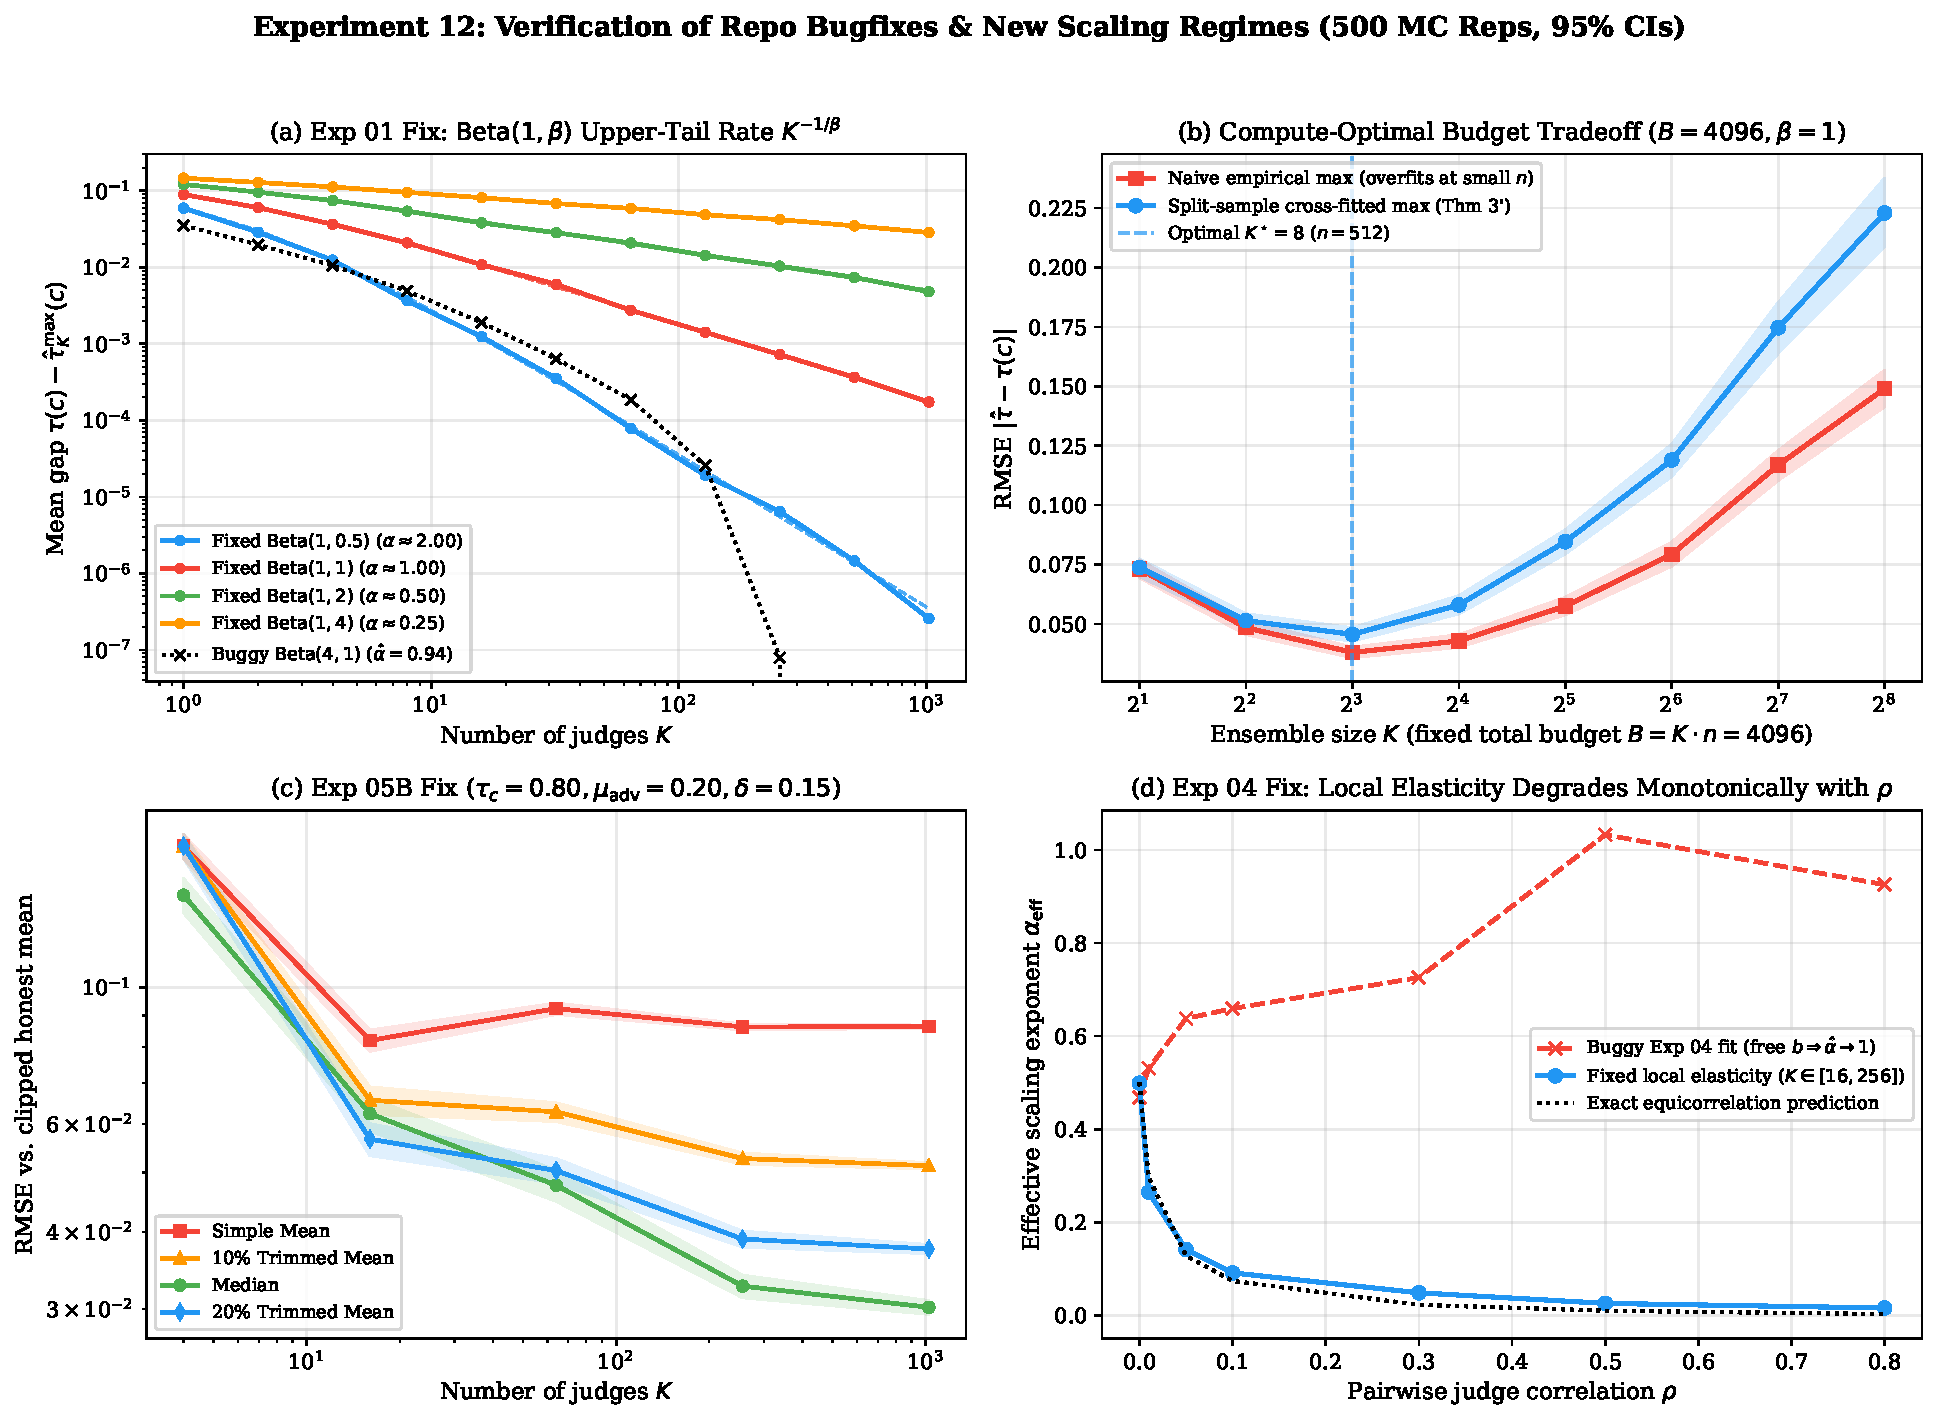
\includegraphics[width=\textwidth]{results/exp12_audit_and_fixes_4panel.pdf}
\caption{Experiment~12 verification across 500 Monte Carlo repetitions with shaded 95\% seed-bootstrap confidence bands (10,000 draws). (a)~Exact $\mathrm{Beta}(1,\beta)$ parameterization restores $K^{-1/\beta}$ decay, contrasting the inverted $\mathrm{Beta}(4,1)$ defect. (b)~Fixed-budget ($B=Kn=4096$, $\beta=1$) error curve showing the interior compute-optimal frontier $K^\star=8, n=512$ for split-sample cross-fitted best-of-$K$. (c)~Non-degenerate contamination ($\tau_c=0.80, \mu_{\mathrm{adv}}=0.20, \delta=0.15$) reveals Simple Mean error saturation vs.\ Median and Trimmed Mean. (d)~Local log-log elasticity ($K \in [16, 256]$) degrades monotonically with correlation $\rho$, eliminating the free-offset $\hat{\alpha} \to 1$ artifact.}
\label{fig:exp12_4panel}
\end{figure}

\subsection{\texorpdfstring{Measured Check A: Prompt-Copy Blindness vs.\ Oriented Peer TVD-MI ($n=400, K=16, 500$ reps)}{Prompt copying and oriented peer scores}}

{\footnotesize\setlength{\tabcolsep}{4pt}
\begin{center}
\begin{tabular}{@{}lcccc@{}}
\toprule
Candidate & Gold Acc. & Prompt TVD-MI & Unsigned Peer TVD-MI & Oriented Peer $\Delta^{\mathrm{orient}}$ \\
\midrule
Oracle & 1.00 & 0.499 [0.499, 0.499] & 0.249 [0.249, 0.250] & $+0.249$ [$+0.249, +0.250$] \\
Noisy Solver & 0.80 & 0.299 [0.297, 0.301] & 0.149 [0.148, 0.150] & $+0.149$ [$+0.148, +0.150$] \\
Prompt-Copier ($Y=X$) & 0.00 & \textbf{0.948} [0.948, 0.948] & 0.020 [0.019, 0.020] & $-0.000$ [$-0.001, +0.001$] \\
Systematic Inverter & 0.00 & 0.499 [0.499, 0.499] & \textbf{0.249} [0.249, 0.250] & $-0.249$ [$-0.250, -0.249$] \\
\midrule
Spearman $\rho$ with Gold & --- & $-0.500$ & $+0.389$ & \textbf{$+0.949$} \\
\bottomrule
\end{tabular}
\end{center}
}

\subsection{\texorpdfstring{Measured Check B: Experiment 01 Bug Fix ($\beta \in \{0.5, 1, 2, 4\}, 500$ reps)}{Corrected coverage simulations}}

{\footnotesize\setlength{\tabcolsep}{3.5pt}
\begin{center}
\begin{tabular}{@{}cccccc@{}}
\toprule
$\beta$ & Theory $1/\beta$ & Buggy $\mathrm{Beta}(\beta,1)$ & Fixed Cont.\ (all $K$) & Fixed Cont.\ ($K \ge 8$ log-log) & Fixed Grid ($K \ge 8$ fit) \\
\midrule
0.5 & 2.0000 & 0.5205 & 1.1475 & \textbf{1.9596} ($R^2=0.9972$) & 1.8750 \\
1.0 & 1.0000 & 0.6975 & 0.7024 & \textbf{0.9871} ($R^2=0.9995$) & 1.0464 \\
2.0 & 0.5000 & 0.8645 & 0.4194 & \textbf{0.4906} ($R^2=0.9981$) & 0.5054 \\
4.0 & 0.2500 & 0.8532 & 0.2270 & \textbf{0.2464} ($R^2=0.9988$) & 0.2588 \\
\bottomrule
\end{tabular}
\end{center}
}

\subsection{\texorpdfstring{Measured Check C1: Null False-Positive Overfitting ($\tau(c)=0, n=50, 500$ reps)}{Null false-positive rates}}

{\footnotesize\setlength{\tabcolsep}{3.5pt}
\begin{center}
\begin{tabular}{@{}ccccc@{}}
\toprule
$K$ & Naive Max Mean [95\% CI] & Split-Sample Mean [95\% CI] & $p$-val (Split $= 0$) & Wilcoxon $p$ ($|$Naive$|$ vs $|$Split$|$) \\
\midrule
1 & $+0.0008$ [$-0.0078, +0.0095$] & $+0.0042$ [$-0.0084, +0.0170$] & 0.657 & $1.75\times 10^{-21}$ \\
16 & $+0.1756$ [$+0.1706, +0.1808$] & $+0.0002$ [$-0.0122, +0.0127$] & 0.698 & $7.96\times 10^{-41}$ \\
64 & $+0.2314$ [$+0.2276, +0.2354$] & $+0.0070$ [$-0.0048, +0.0188$] & 0.172 & $4.59\times 10^{-75}$ \\
256 & $+0.2744$ [$+0.2711, +0.2778$] & $+0.0068$ [$-0.0050, +0.0189$] & 0.176 & $2.45\times 10^{-81}$ \\
1024 & \textbf{$+0.3155$} [$+0.3122, +0.3189$] & \textbf{$+0.0063$} [$-0.0058, +0.0184$] & 0.448 & $7.60\times 10^{-83}$ \\
\bottomrule
\end{tabular}
\end{center}
}

\subsection{\texorpdfstring{Measured Check D ($K=1024$) and Check E ($K \in [16, 256]$)}{Large-panel median bias and local scaling}}

\textbf{Check D ($\tau_c=0.80, \mu_{\mathrm{adv}}=0.20, \sigma=0.20, \delta=0.15, K=1024$):}
Simple Mean RMSE $= 0.0863$ [$0.0858, 0.0868$] (bias $-0.0861$);
$10\%$-Trimmed Mean RMSE $= 0.0513$ [$0.0507, 0.0519$] (bias $-0.0509$, $p = 1.26\times 10^{-83}$ vs.\ Mean);
$20\%$-Trimmed Mean RMSE $= 0.0375$ [$0.0369, 0.0382$] (bias $-0.0369$, $p = 1.26\times 10^{-83}$);
Median RMSE $= 0.0302$ [$0.0294, 0.0309$] (bias $-0.0289$, $p = 1.26\times 10^{-83}$, bounded by unclipped Huber shift $-0.0446$).

\textbf{Check E ($\sigma^2=0.1$ equicorrelated RMSE elasticity over $K \in [16, 256]$):}
Broken free-offset \texttt{fit\_power\_law} jumps $\rho=0 \to 0.50$: $0.4681 \to 1.0325$;
Fixed local elasticity drops monotonically as predicted: $\rho=0.00 \Rightarrow 0.4990$ (theory $0.5000$), $\rho=0.01 \Rightarrow 0.2647$ (theory $0.2967$), $\rho=0.05 \Rightarrow 0.1418$ (theory $0.1282$), $\rho=0.10 \Rightarrow 0.0915$ (theory $0.0743$), $\rho=0.30 \Rightarrow 0.0487$ (theory $0.0229$), $\rho=0.50 \Rightarrow 0.0260$ (theory $0.0102$), $\rho=0.80 \Rightarrow 0.0160$ (theory $0.0026$).

\subsection{Ranked Roadmap for Next Experiments (Ordered by Decision Value)}

\begin{enumerate}[leftmargin=*,itemsep=3pt]
\item \textbf{[Priority 8/10] Experiment 13 — Real Multi-LLM Judge TVD-MI Scaling on Public Cached Corpora (\texttt{SummEval} \& \texttt{HelpSteer2}):} Reuse zero-cost archived scores (e.g.\ SummEval 1,600 summaries $\times$ 20 G-Eval completions + BARTScore/ROUGE metrics, and public HelpSteer2 ordinal panels) to replace Experiment~06's synthetic Gaussian proxy with real correlated LLM ensembles, testing oriented conditional peer TVD-MI, prompt-copy stress tests, split-sample $K^\star(B)$, and residual pairwise error correlation $\hat{\rho}_K$ vs.\ Experiment~04's floor. \emph{Currently untested on real LLM text outputs.}
\item \textbf{[Priority 8/10] Experiment 14 — Cross-Item Spectral / Dawid--Skene / IRT Calibration Under Correlated Confounders \& $\delta > 0.2$:} Test whether spectral initialization + EM over $n \times K$ candidate--judge matrices eliminates the single-item $O(\sigma\delta)$ median shift and survives adversarial fractions up to $\delta < 1/2$ even under shared confounders $W$ (Theorem~\ref{thm:confounded_consensus}).
\item \textbf{[Priority 7/10] Paper \& Historical Script Reconciliation:} Fix the four bugs directly inside \path{experiments/01_basic_scaling_law/}, \path{03_two_axis_decomposition/}, \path{04_diversity_dependence/}, \path{05_adversarial_robustness/}, \path{07_aggregation_rules/}, and \path{11_finite_sample_bounds/} (recording pre/post versions cleanly), update \path{latex_paper/neurips/05_two_axis_decomposition.tex} ($2e^{-n\eta^2}$), \path{10_experiments.tex}, and \path{98_appendix_experiments.tex}, and populate the paper with verified figures and real-LLM curves.
\item \textbf{[Priority 7/10] Lean 4 Finite-PMF TVD Duality \& Concentration Upgrade (\path{experiments/00_lean_formalization/}):} Formalize finite-PMF variational TVD duality, Theorem~\ref{thm:oriented_peer} (bijection invariance), and Theorem~\ref{thm:split_thm3p} (split-sample concentration) in \path{TvdmiJudge/FiniteTVD.lean}.
\item \textbf{[Priority 6/10] Optimal Non-Uniform Judge Selection \& Cost-Aware Ensembles:} Study optimal $K$ sizing when judges vary in cost ($c_j$) and competence ($\gamma_j, \rho_{ij}$), testing Nitzan--Paroush optimal log-odds weights vs.\ uniform majority vote under finite anchor budgets.
\end{enumerate}

\section*{Sources}
\begin{itemize}[leftmargin=*,itemsep=2pt]
\item Repository audited: \path{brando90/tvdmi-judge-asymptotics} (\path{experiments/00_lean_formalization/}--\path{experiments/11_finite_sample_bounds/}, \path{latex_paper/neurips/main.tex}, \path{theory/assumptions.md}).
\item Experiment~12 verification code \& raw CSVs: \path{experiments/12_repo_audit_bugfixes_and_next_theory_roadmap_start_21Nov2026/run_audit_and_verifications.py} and \path{results/{checkA..checkE,summary_metrics.json}}.
\item Lean~4 verification: \texttt{lake build} on Lean~v4.29.0 (\texttt{3287} jobs) + \texttt{\#print axioms} check in \path{experiments/00_lean_formalization/lean/}.
\item Base framework citations: Robertson \& Koyejo (ICML~2025, TVD-MI finite-sample/adversarial robustness); Robertson \& Koyejo (2025, TVD-MI score matrices via IRT); Chen et al.\ (2026, CARE confounded multi-judge aggregation).
\end{itemize}

\end{document}
